\section{Alternate PSF Fitting Configurations}
\label{app:alternate_configs}
\subsection{Spatial Order 2, Colour Order 1}
This section shows plots with the following fitting configuration.
We use the same spatial order as Sec.~\ref{sec:results} but reduce the colour order from 2 to 1.
\lstinputlisting[language=Python]{finalizeCharacterizationConfig_colororder1.py}

\begin{figure}[h!]
  \centering

  \begin{subfigure}{\textwidth}
    \centering
    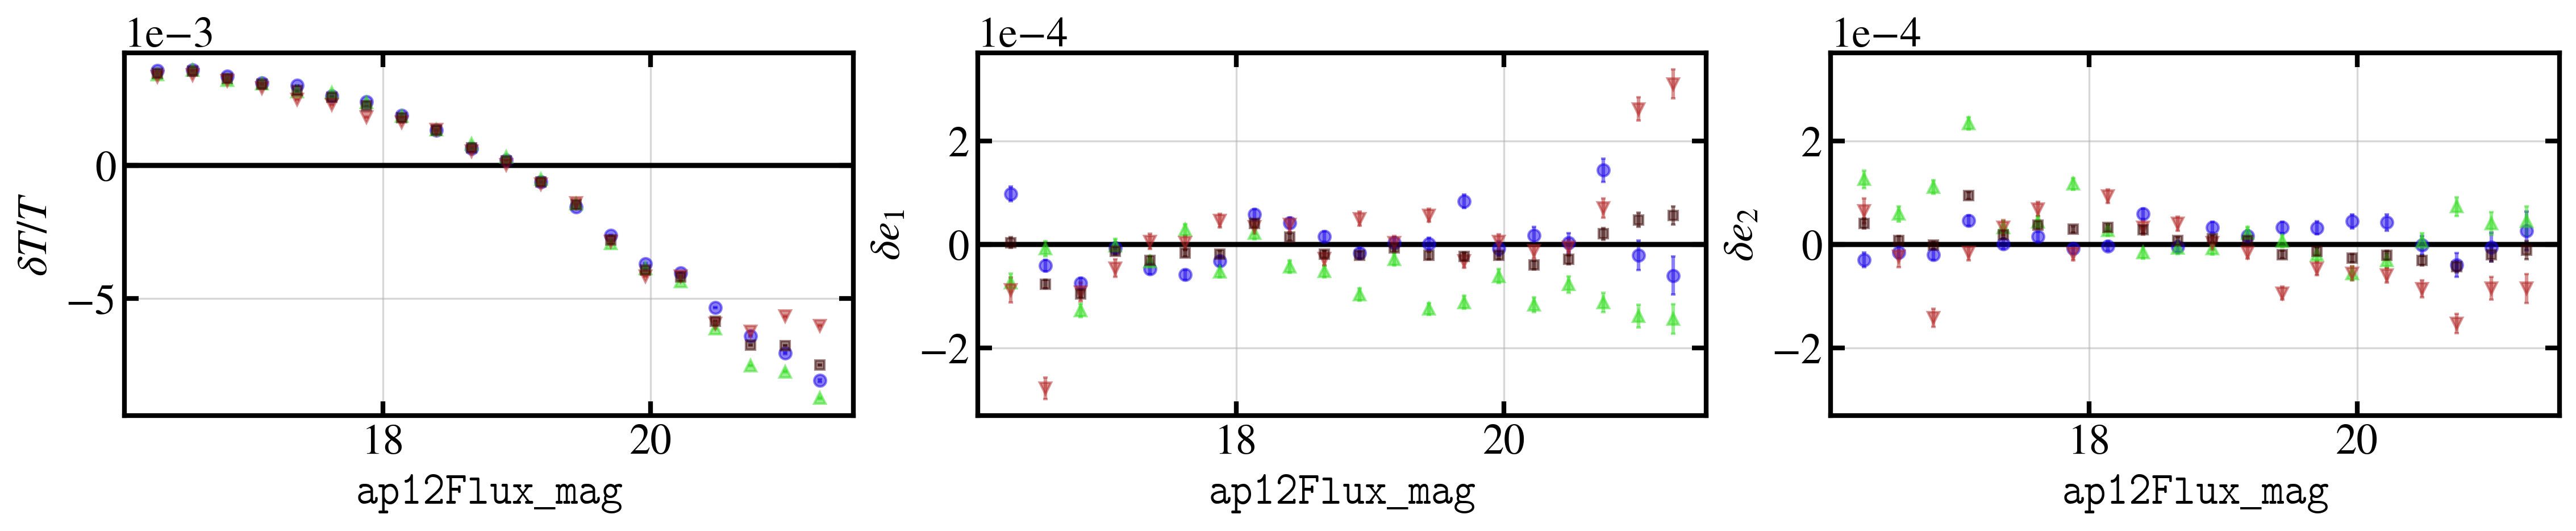
\includegraphics[width=1\textwidth]{figures_colororder1/color_separated_residuals_vs_calibfluxmag_with_correction_20260411.png}
    \caption{PSF residuals across all bands vs. magnitude, with chromatic fitting.}
  \end{subfigure}
  \medskip
  \begin{subfigure}{\textwidth}
    \centering
    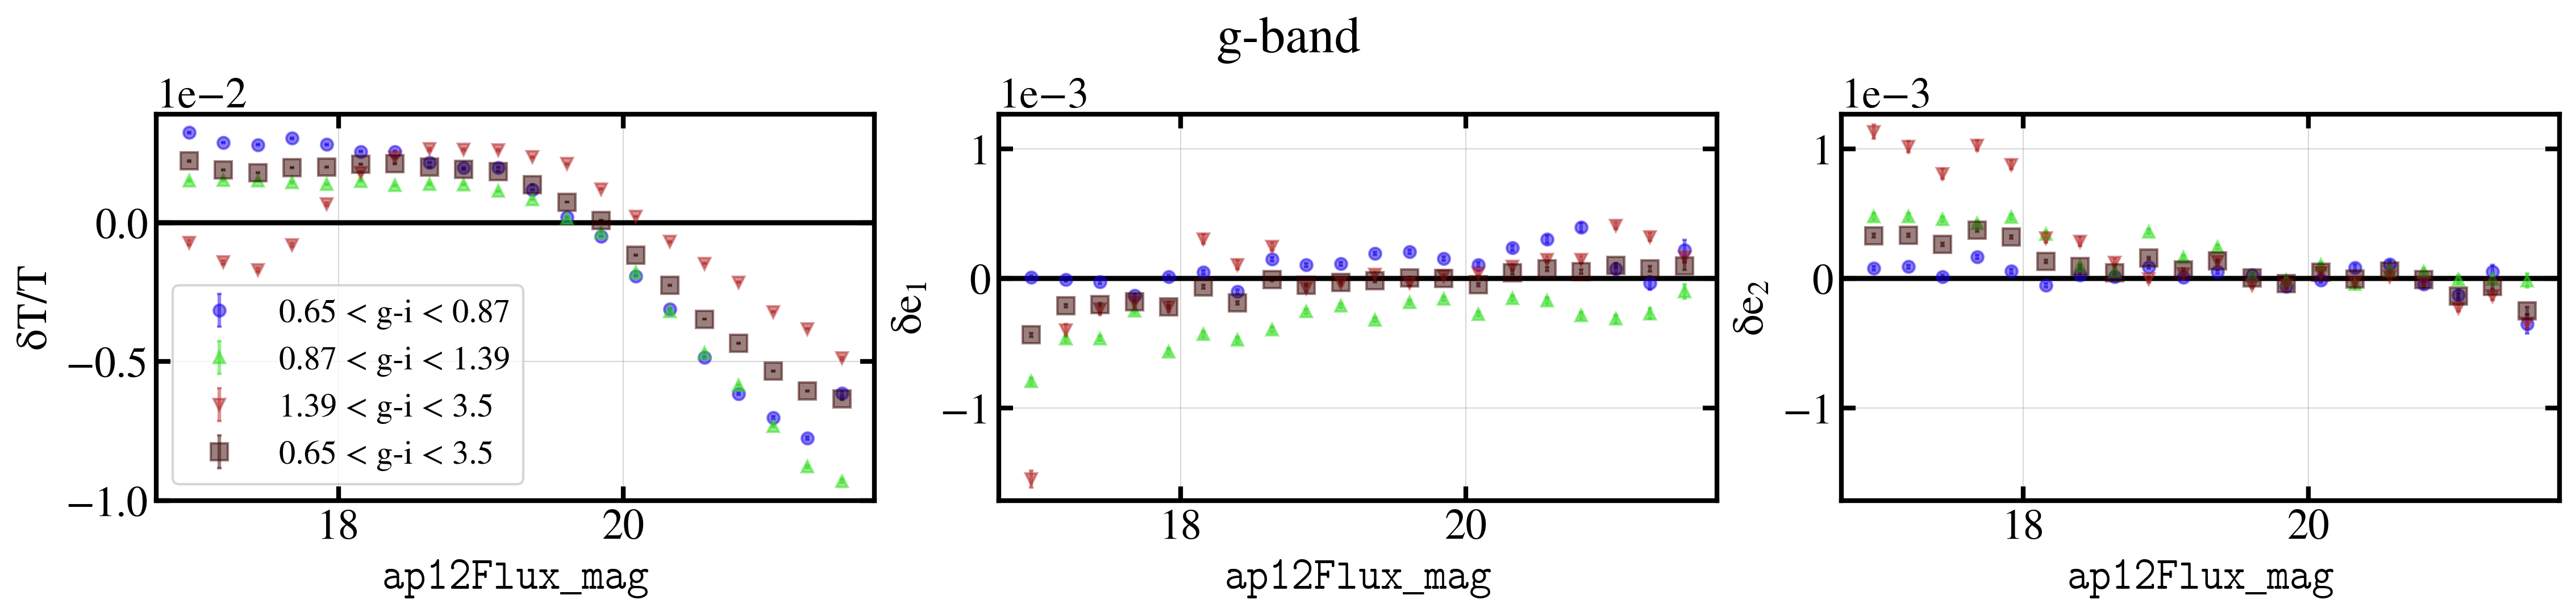
\includegraphics[width=1\textwidth]{figures_colororder1/color_separated_residuals_vs_calibfluxmag_with_correction_g_band_20260411.png}
    \caption{{\it g} band PSF residuals vs. magnitude, with chromatic fitting.}
    \label{subfig:residuals_vs_mag_g_colororder1}
  \end{subfigure}
  \caption{Residuals as a function of \texttt{ap12Flux\_mag} after chromatic fitting with colour order 1.
  Stars are divided into equal-sized colour bins of $g-i \in [0.65, 0.87, 1.39, 3.5]$.
  There are no significant differences between this configuration and the configuration used in Subfigs.~\ref{subfig:residuals_vs_mag_b} and \ref{subfig:residuals_vs_mag_g_b}.}
    \label{fig:residuals_vs_mag_colororder1}
\end{figure}

\begin{figure}[h!]
  \centering

  \begin{subfigure}{\textwidth}
    \centering
    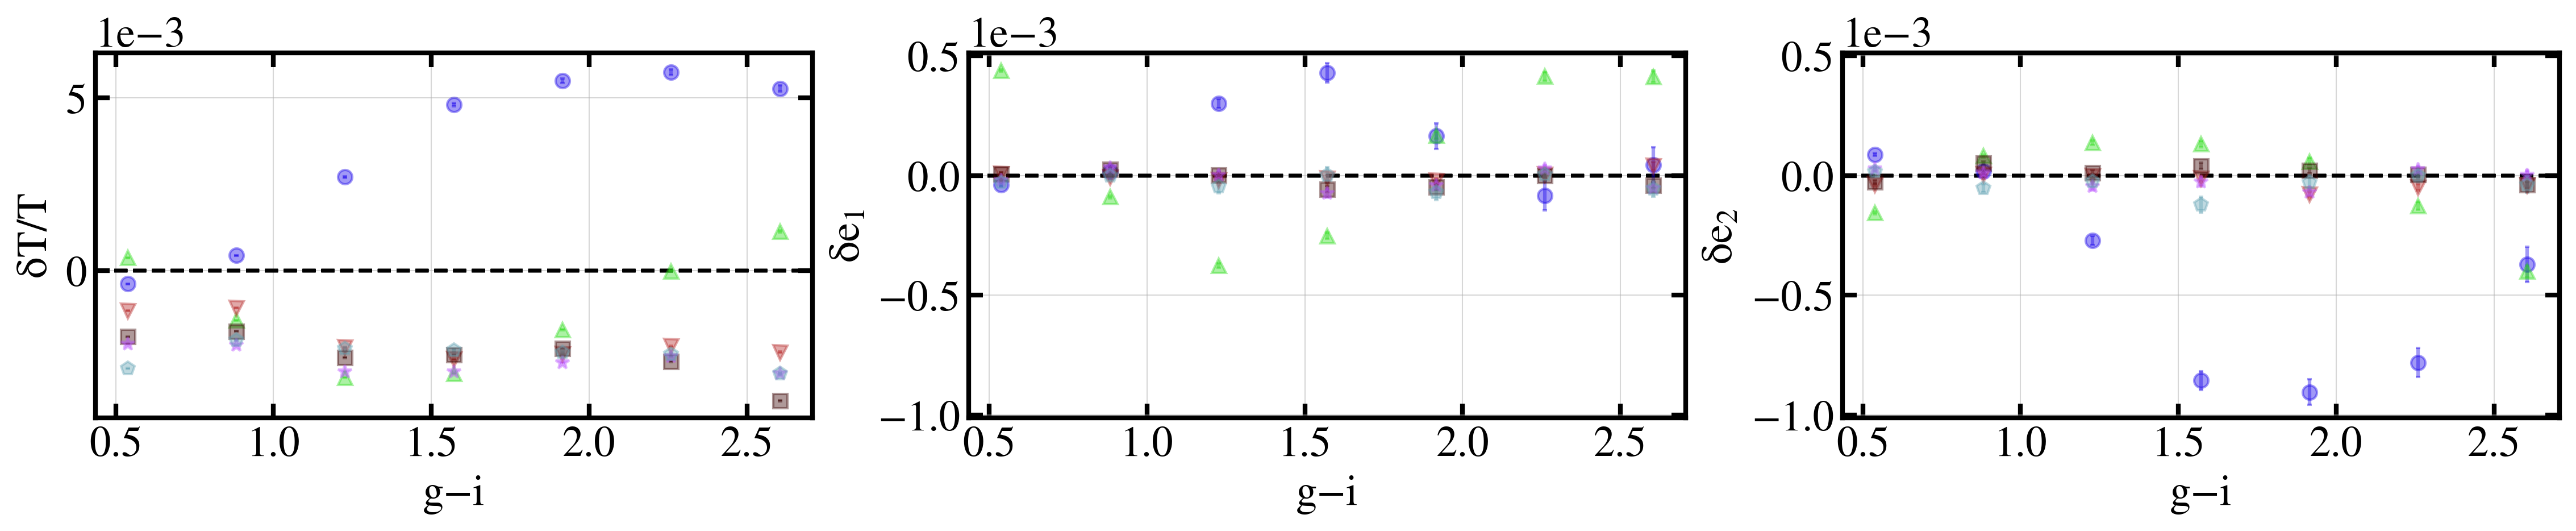
\includegraphics[width=1\textwidth]{figures_colororder1/residuals_vs_gmi_color_with_correction_20260411.png}
    \caption{with chromatic PSF fitting.}
  \end{subfigure}
  \medskip
  \begin{subfigure}{\textwidth}
    \centering
    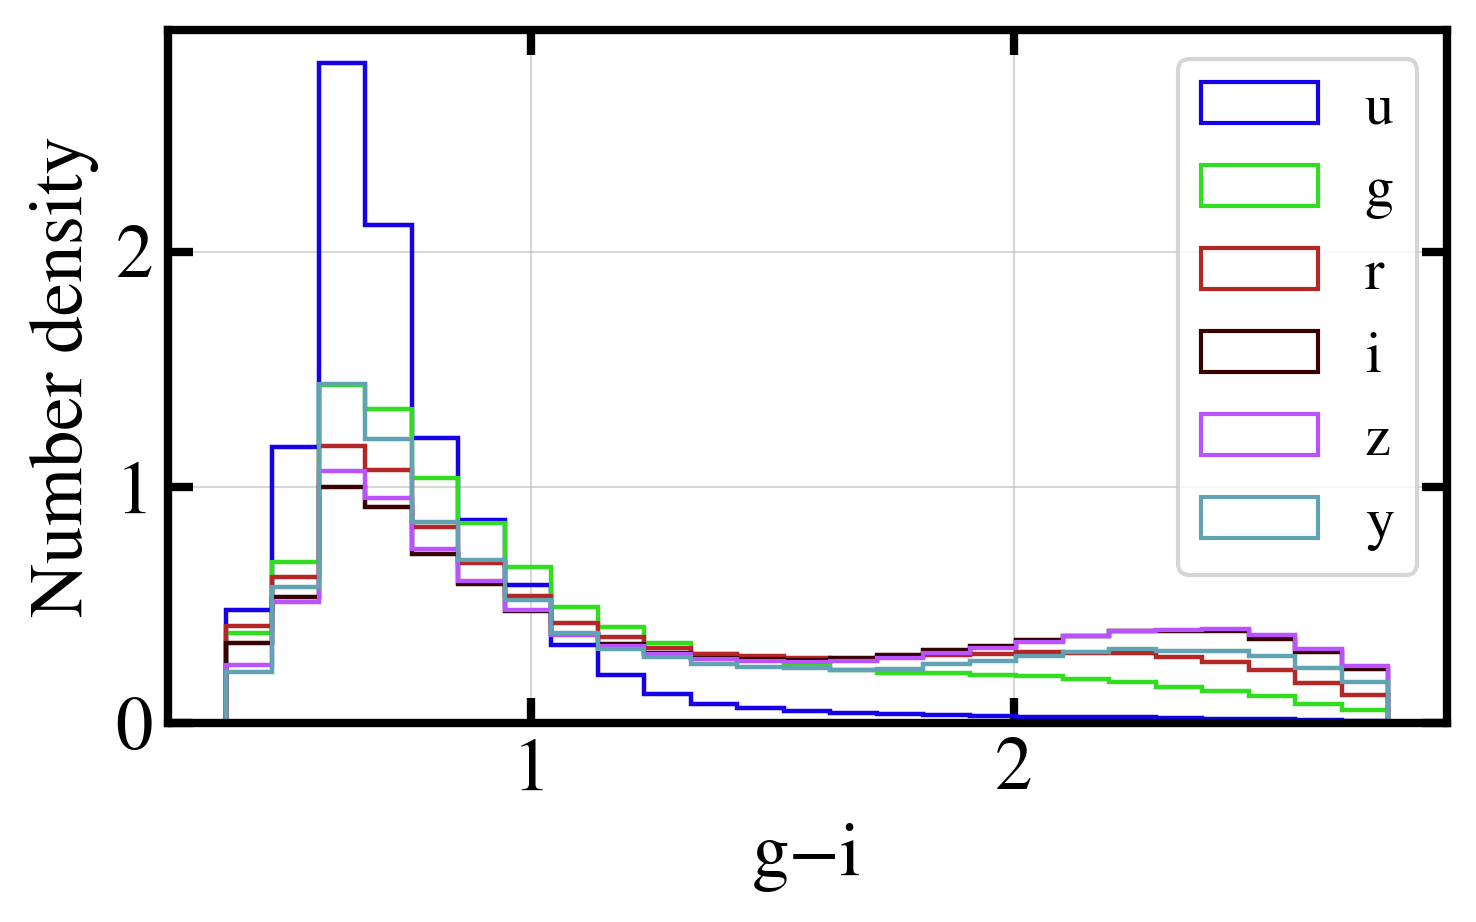
\includegraphics[width=0.3\textwidth]{figures/color_hist.png}
    \caption{Number density as a function of $\textit{g}-\textit{i}$ colour.}
  \end{subfigure}

  \caption{PSF residuals as a function of $\textit{g}-\textit{i}$ colour. 
  The {\it u} and {\it g} band residuals show the highest dependence on $\textit{g}-\textit{i}$ colour. 
  The {\it g} band residual is not corrected as well here as it is with colour order 2 in Subfig.~\ref{subfig:color_vs_residuals_b}. }
  \label{fig:residuals_vs_colour}
\end{figure}

\begin{figure}[h!]
  \centering

  \begin{subfigure}[t]{0.45\textwidth}
    \centering
    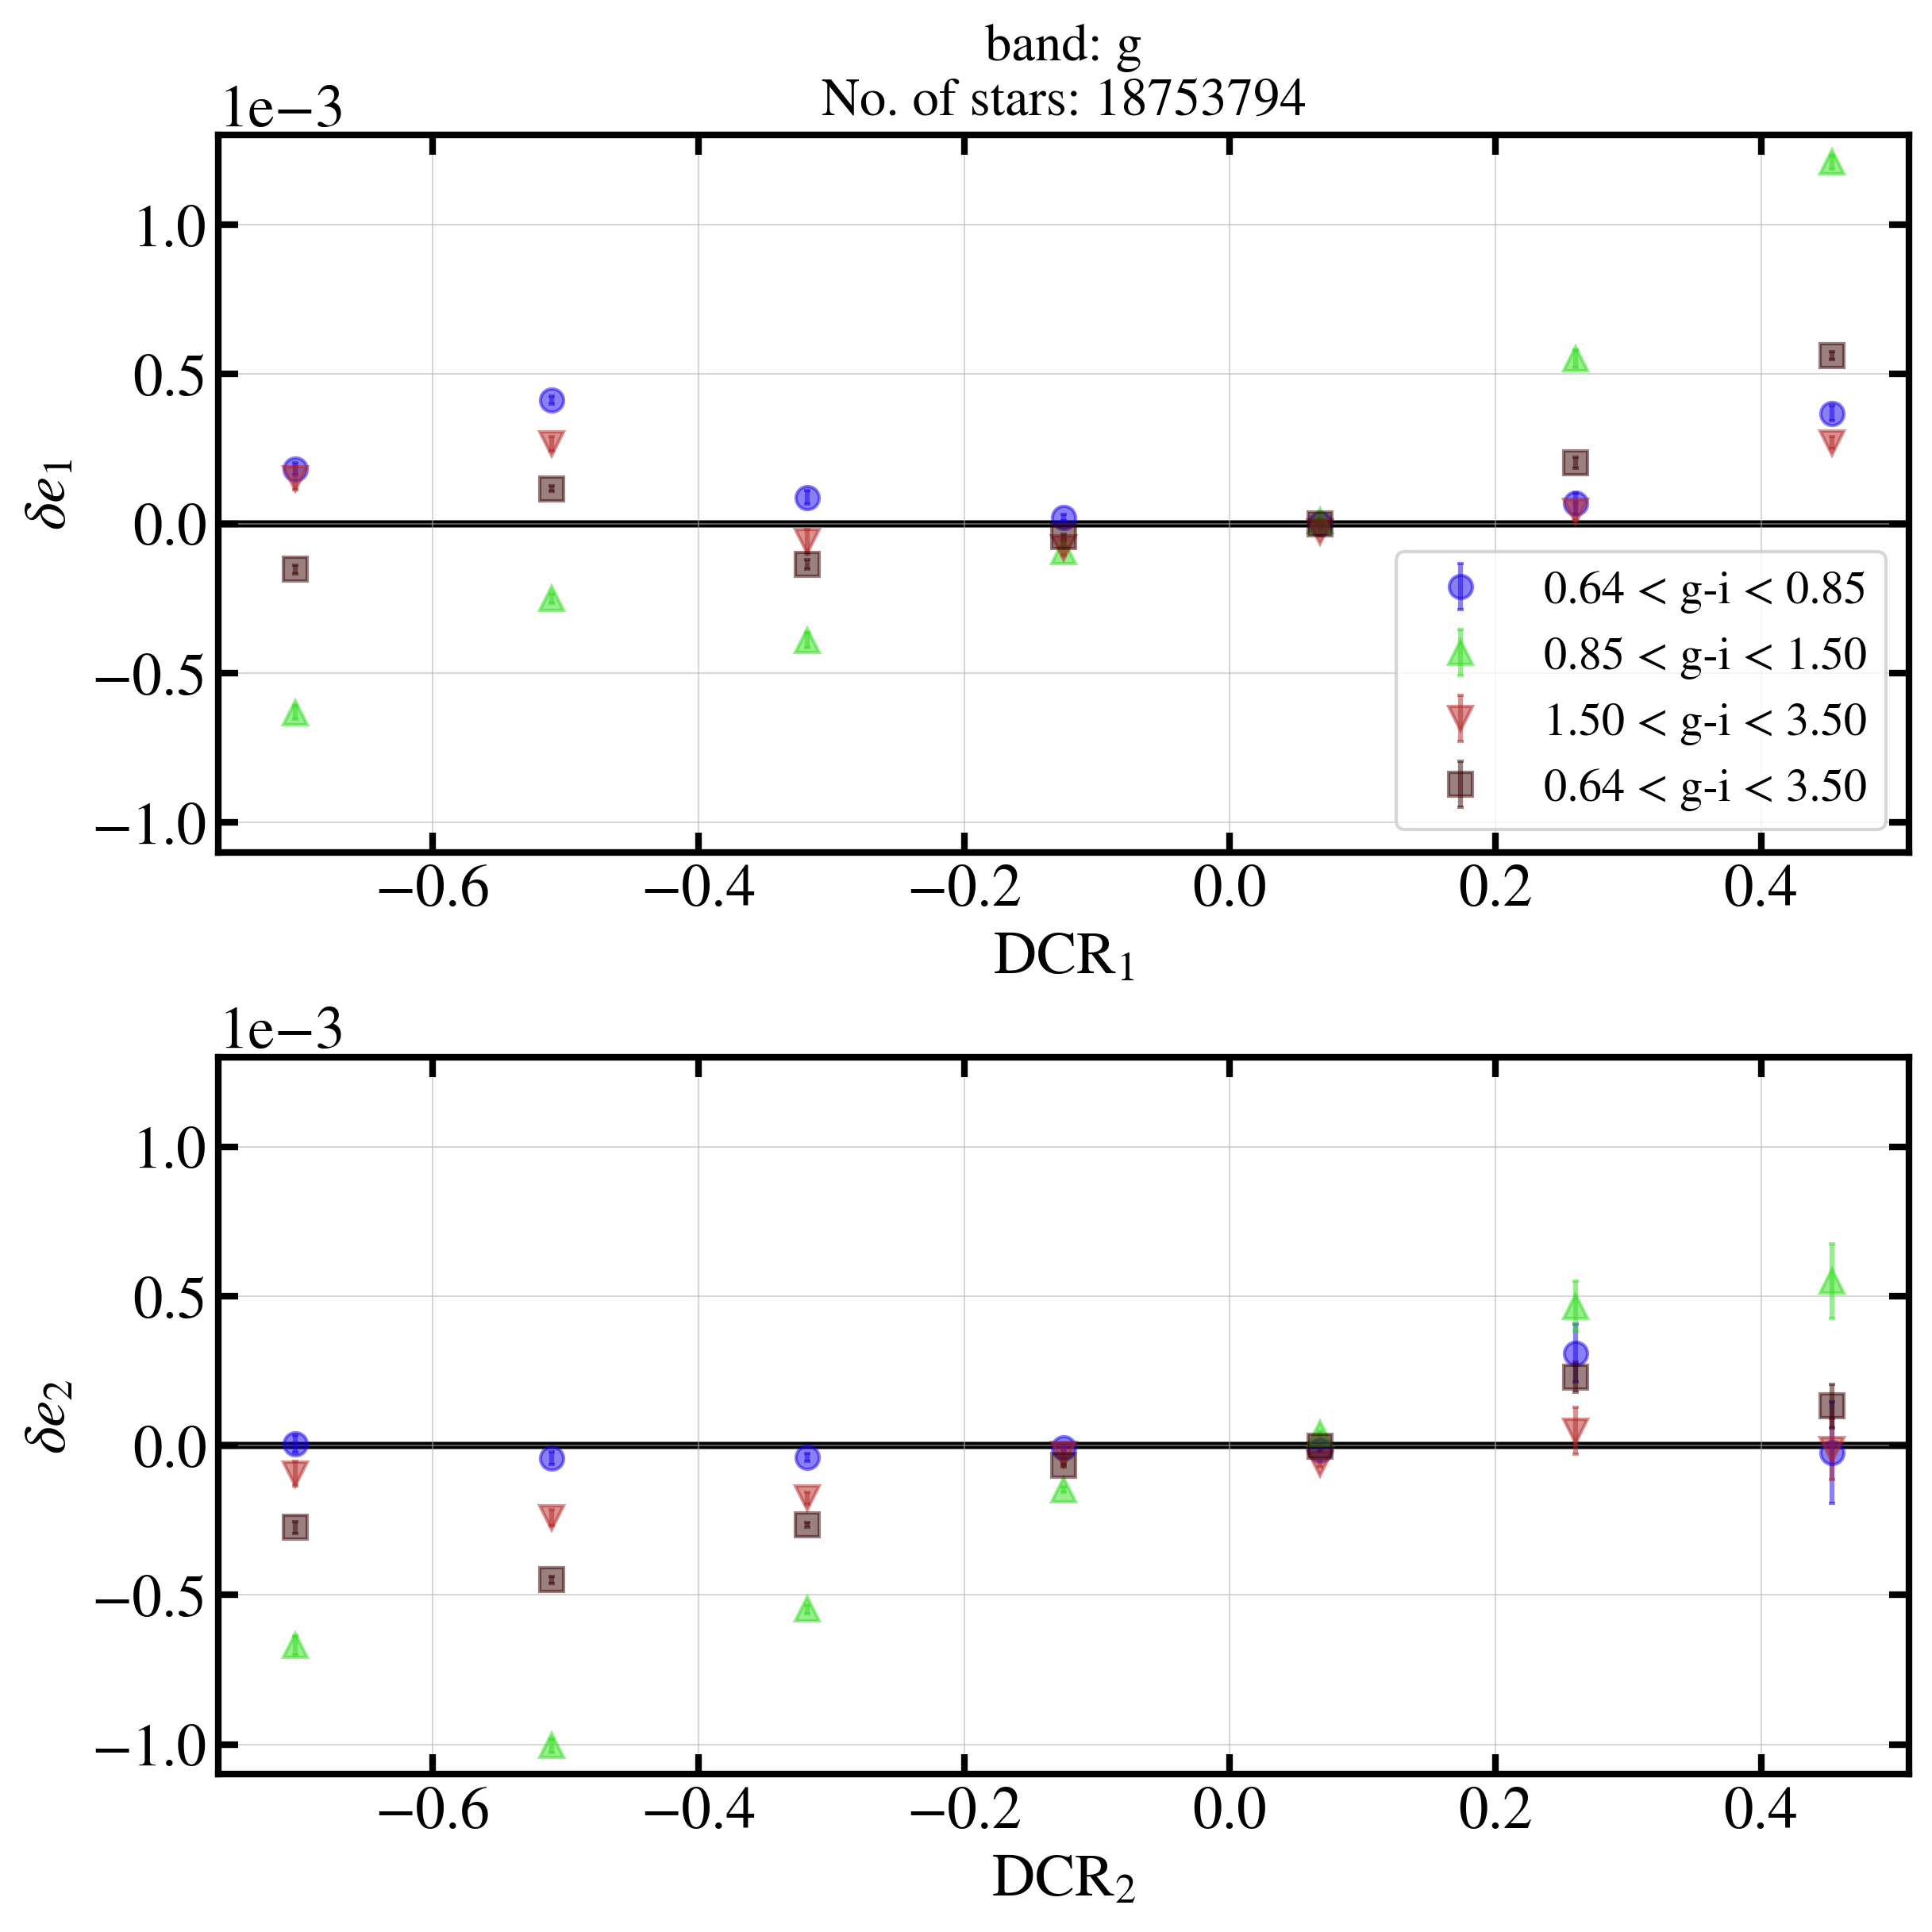
\includegraphics[width=\linewidth]{figures_colororder1/shape_residuals_vs_dcr_g_with_correction_20260411.png}
    \caption{DCR in the {\it g} band after chromatic fitting.}
    \label{subfig:g_dcr_colororder1}
  \end{subfigure}
  \hfill
  \begin{subfigure}[t]{0.45\textwidth}
    \centering
    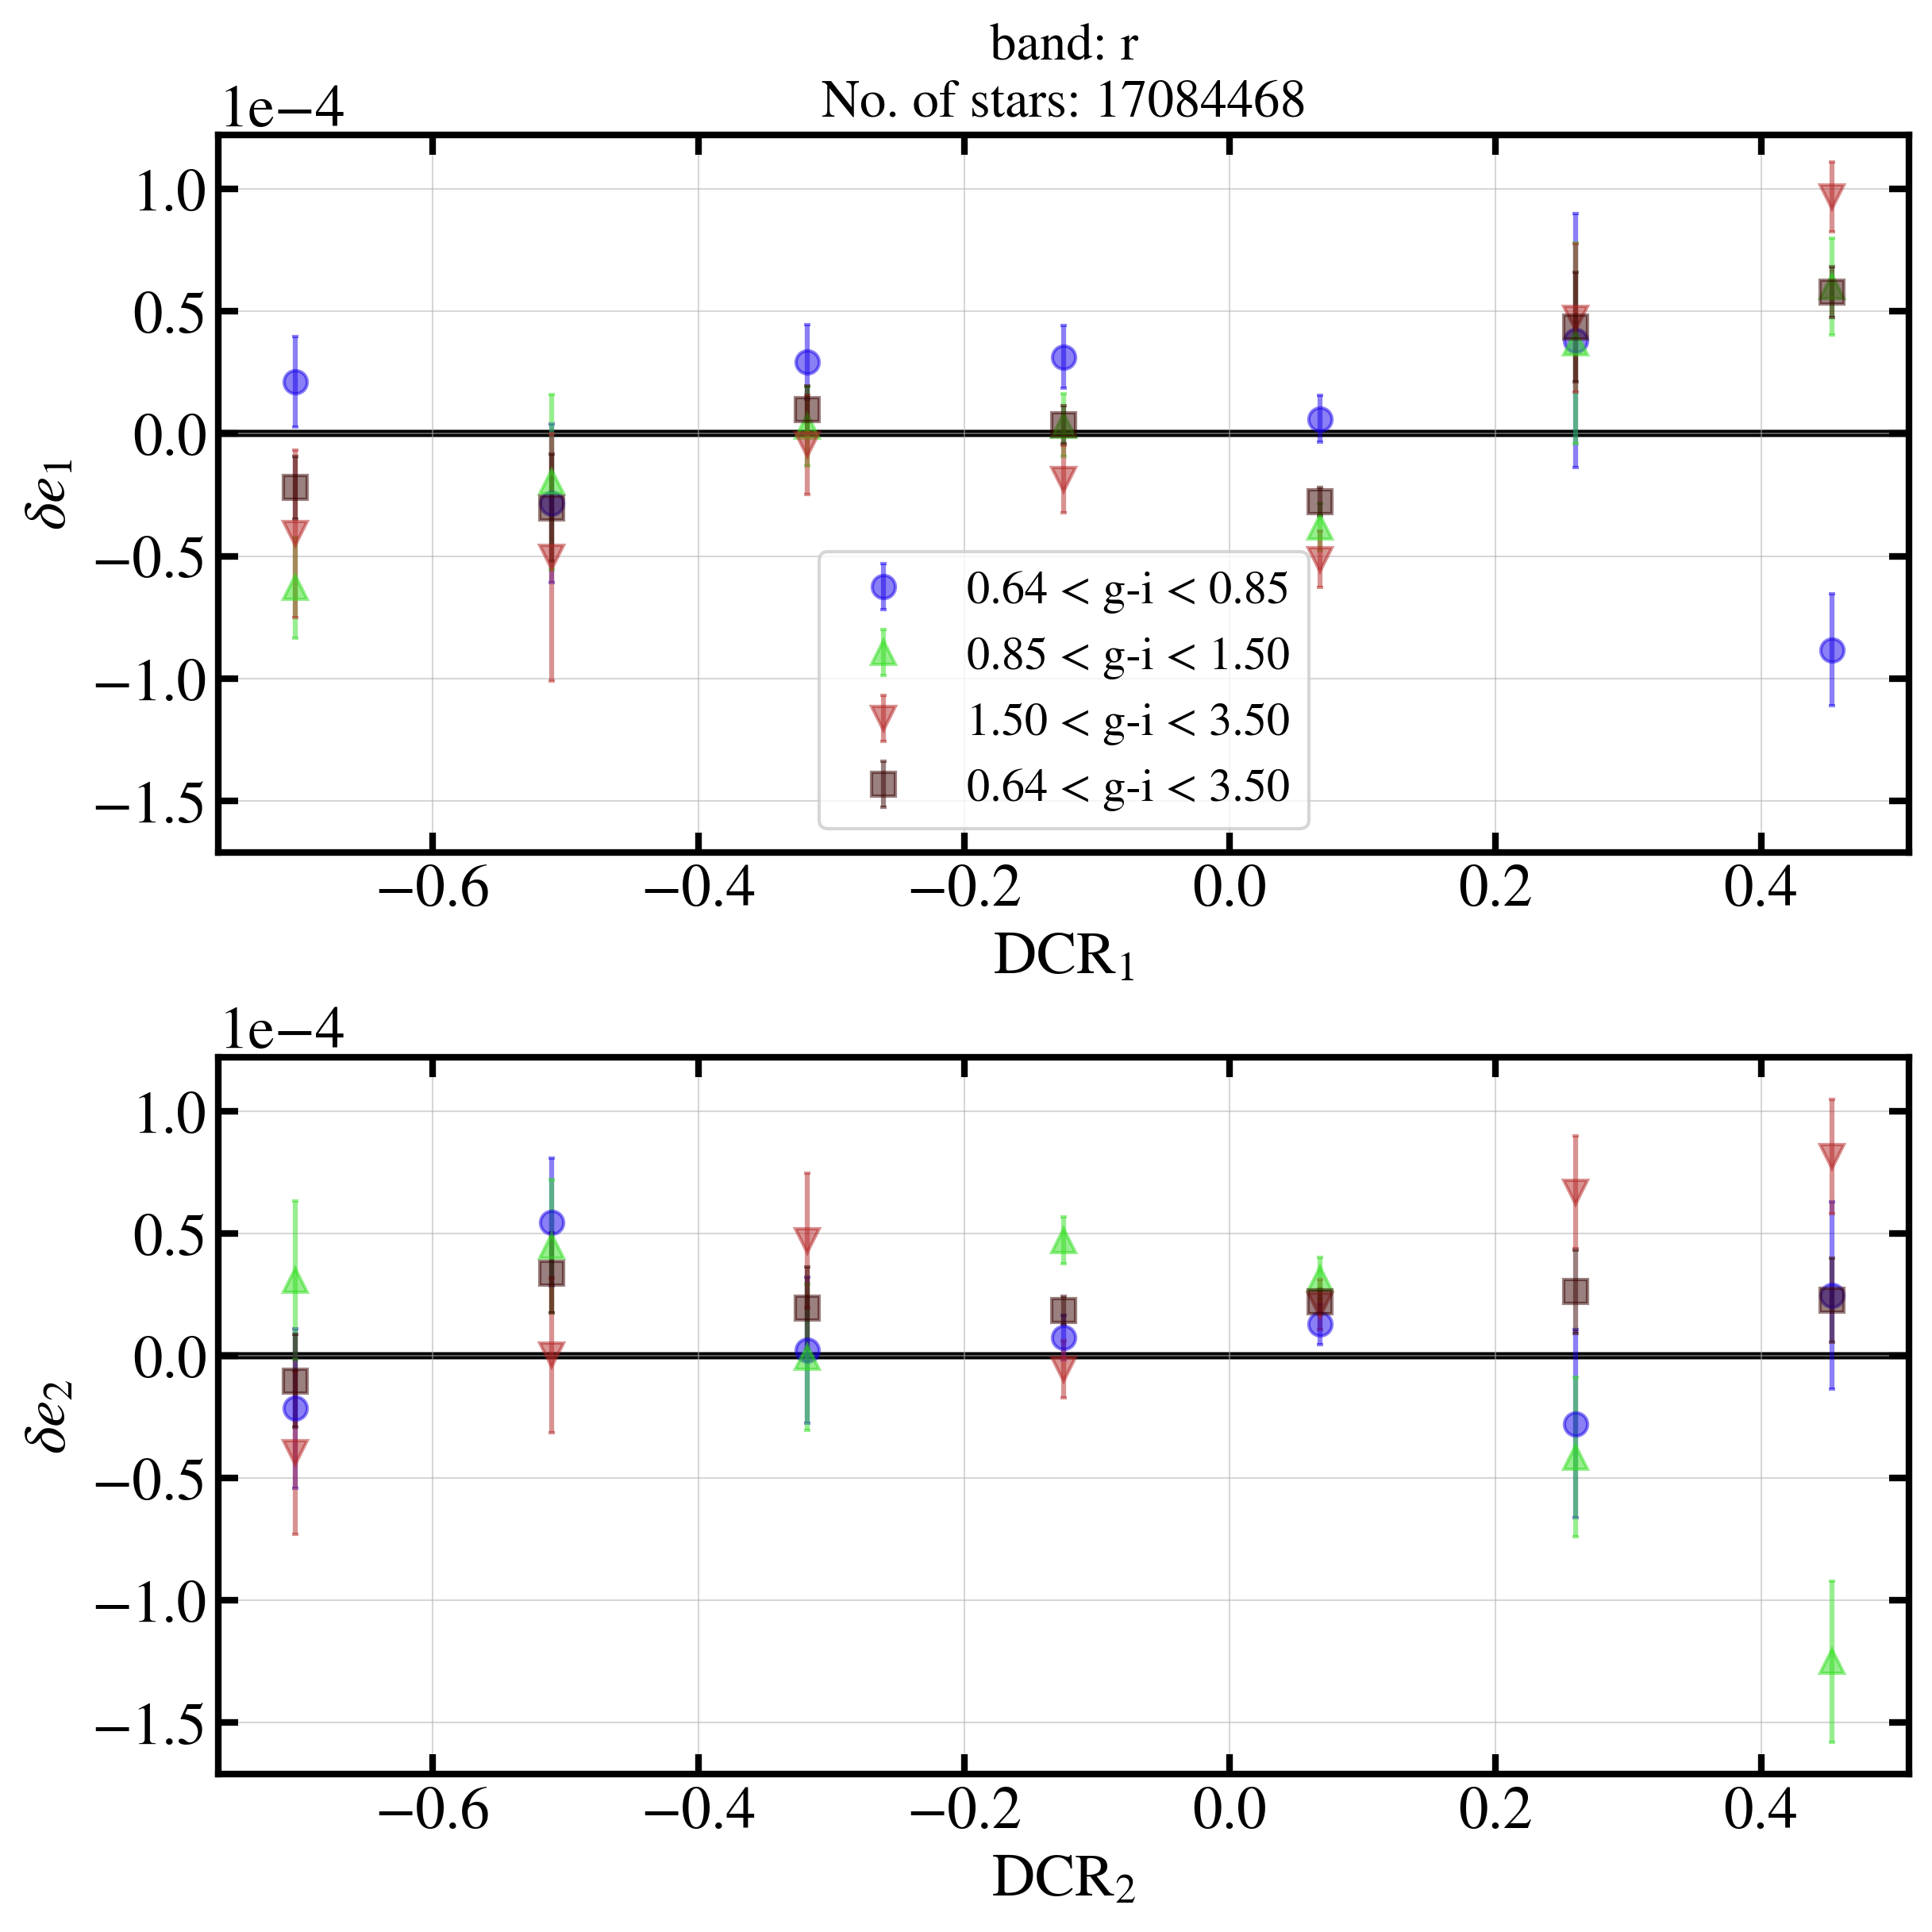
\includegraphics[width=\linewidth]{figures_colororder1/shape_residuals_vs_dcr_r_with_correction_20260411.png}
    \caption{DCR in the {\it r} band after chromatic fitting.}
    \label{subfig:r_dcr_colororder1}
  \end{subfigure}

    \caption{PSF $\delta e_1$ and $\delta e_2$ as a function of $\mathrm{DCR_1}$ and $\mathrm{DCR_2}$. 
   Residuals in the {\it g} band are $\sim$50\% larger than when using colour order 2 in Subfig.~\ref{subfig:g_dcr_b}.
   Residuals in the {\it r} band are on a comparable level to those in Subfig.~\ref{subfig:r_dcr_b}.}
  \label{fig:dcr_colororder1}
\end{figure}
